\begin{tikzpicture}
\node [mybox] (box){%
    \begin{minipage}{0.3\textwidth}
    \newcommand{\warning}[1]{\textcolor{red}{\footnotesize\textit{#1}}}
    \begin{tabular}{p{0.3\textwidth} p{0.61\textwidth}}
      \vspace{-10pt}\hspace{-0.85cm} 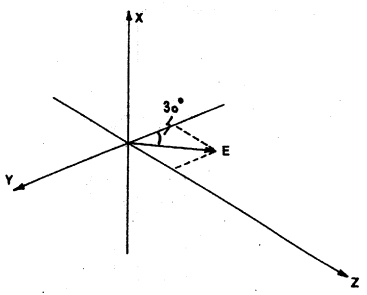
\includegraphics[scale=0.25]{images/ex_optique_physique.png} &
      \vspace{-8pt} {
          \txt{\textit{
          Un laser émet un faisceau lumineux de rayon $r_L=1cm$ selon l'axe X négatif. Fréquence $f=10^{12}Hz$. Champ électrique possède une amplitude $E_o=10^5 V/m$. \textbf{a)} Expression de l'OEM E et B?
          \textbf{b)} Laser frappe en son centre une plaque métallique avec un coeff. de réflexion $R=0.4$; $m=0.5$ grammes; diamètre $d_p=1cm$. Temps écoulé en heures si un observateur situé sur la plaque métallique mesure un $\lambda_o$ qui diffère de 0.8nm de celle émise par le laser $\lambda_s$? Hypothèse: $v<<c$.}
          }
      }
    \end{tabular}
    \txt{
        \def \w {2\cdot 10^{12}\pi}
        \def \k {2.1\cdot10^4}
        
        \textbf{a)} $f=10^{12}Hz$, $E_o=10^5V/m$\\
        $\rightarrow$ $\boxed{\omega=2\pi f}=2\cdot \pi \cdot 10^{12}=2\times 10^{12}\pi$ rad/s\\
        $\rightarrow$ $\boxed{k=\omega/c}=\omega\cdot3\times 10^8=2.095\times10^4$ rad/m\\
        $\Vec{S}$ se propage vers z < 0 donc $E=E_ocos(\omega t - k z)$ (angle \textit{cos} rapport à z)\\
        \textbf{Pour le champ électrique $E$:}\\
        $\rightarrow$ $E_x=0$ V/m \textbf{et} $E_y=(-)E_o\cdot cos 30^\circ$\warning{*} V/m \textbf{et} $E_z=E_o cos 60^\circ$ V/m\\
        \dbox{$E(z,t)=[0\ _i E_y\ _j + E_z\ _k] cos (\w t + \k z)\ V/m$}\warning{**}
        
        \warning{*TOUJOURS REGARDER la direction sur l'axe pour les signes négatif}\\
        \warning{**Angle du vecteur E cos par rapport à Z}
        
        \textbf{Pour le champ magnétique $B$:}
        $\boxed{c=\frac{E_o}{B_o}}\Rightarrow B_o=3.3\cdot 10^{-4}$ Tesla\\
        $\rightarrow$ $B_x=0$ V/m \textbf{et} $B_y=B_o\cdot sin 30^\circ$ V/m \textbf{et} $B_z=B_o cos 30^\circ$ V/m\\
        $\rightarrow$ \dbox{$B(z,t)=[0\ _i B_y\ _j + B_z\ _k] cos (\w t + \k z)\ V/m$} T \warning{*}\\
        \warning{*Angle du vecteur B cos par rapport à Z}
        
        \textbf{b)} $R=0.4$, $m=0.5g$, $r_L=1cm$, $d_p=1cm$, $\Delta\lambda=0.8nm$\\
        \textbf{Selon x:} $\boxed{\vec{v}=\vec{v_s}-\vec{v_o}}=0-(-\vec{v_o})=\vec{v_o}$\\
        $\vec{v}>0 \Rightarrow$ donc éloignement relatif et $f_o<f_s$\\
        \warning{*Faire graphique AVEC la direction du x. Laser fait de la pression de radiation sur la plaque (obs) qui se déplace et le laser (src) est immobile par rapport à l'obs.}\\
        $\rightarrow$ $\boxed{c=\lambda_s/f_s}\Rightarrow\ 3\cdot  10^8=\lambda_s\cdot 10^12\Rightarrow \lambda_s=3\cdot 10^{-4}$\\
        $v<<c$ donc $v/c<<1$ alors $\boxed{\Delta \lambda/\lambda_s=1+\frac{v}{c}cos\theta-1}$\\
        $\rightarrow$ $solve(\frac{0.8\cdot 10^{-9}}{3\cdot 10^{-4}}=1+\frac{v}{3\cdot 10^8} cos 0^\circ, v) \Rightarrow$ \dbox{$v_o=800.25$ m/s}\\
        $\rightarrow$ $\boxed{P=\frac{(R+1)}{c}I=\frac{F}{A_\bot}} \Rightarrow \boxed{F=ma}=0.0005kg\cdot a$\\
        $\Rightarrow \boxed{I=\frac{E_o\ B_o}{2\_\mu_o}}=1.33\cdot 10^{-7} \Rightarrow \boxed{A_\bot} = \pi (d_p/2)^2=0.79cm^2$\\
        $\Rightarrow solve(\frac{(R+1)}{\_c}I=\frac{m\cdot a}{A_\bot \_cm}, a) \Rightarrow a=0.0097 m/s^2$ \warning{*Attention cm vs. m}\\
        $\boxed{v_f=v_i+a\Delta t}=800=0+0.001 \cdot \Delta t \Rightarrow \Delta t = 800000s = 222 heures$
        
    }
    \end{minipage}
};
\node[fancytitle, right=10pt] at (box.north west) {Exercice optique physique};
\end{tikzpicture}